\section{Апробация и анализ результатов}\label{appob}
В данной главе представлены результаты апробации алгоритмов из \emph{библиотеки алгоритмов полулокальных задач}.
Также дана оценка применимости решений полулокальных задач \emph{semi-local lcs и sa} к поиску групп повторов в \emph{JavaDoc}-комментариях и задаче поиска повторов по шаблону.


\subsection{Тестовый стенд}
Для проведения экспериментов использовалась
машина с процессором \emph{Intel-Core i5} и оперативной памятью размером \emph{16GB}.
Операционная система \emph{Ubuntu 18.04 Bionic}.
На каждый запуск \emph{jar}-файла выделялось $10GB$ памяти.

\subsection{Экспериментальная проверка асимптотики}
В данной секции описаны экспериментальные результаты запусков части алгоритмов из реализованной \emph{библиотеки алгоритмов} (см. главу \ref{librarySection})  и дана их интерпретация.

На рис. \ref{fig:speedlcs} представлен результат запусков
обычного \emph{prefix lcs}, \emph{prefix lcs} с хранением результатов с помощью одной строки и полулокального \emph{lcs} (\emph{semi-local lcs reducing}).
\begin{figure}[h]
\centering
    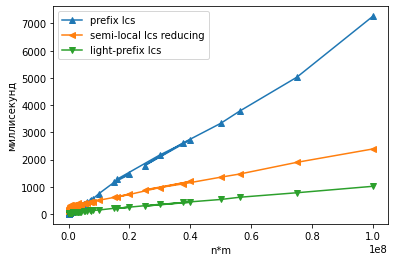
\includegraphics[width=0.6\columnwidth]{figures/semiLocalvsPrefixLCS.png}
    \caption{Результат запусков различных версий подсчета \emph{lcs} }\label{fig:speedlcs}
\end{figure}
Исходя из результатов, можно сделать вывод, что скорость вычисления \emph{semi-local lcs} сопоставима с вычислением обычного \emph{lcs}.


На рис. \ref{fig:speedlcs2} представлено сравнение двух реализаций подсчета \emph{semi-local lcs}: через распутывание кос (\emph{reducing}) и  умножение кос (\emph{recursive}).
\begin{figure}[H]
\centering
    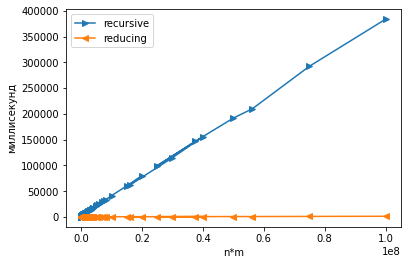
\includegraphics[width=0.6\columnwidth]{figures/semilocalReducignVssemiLocalRecursive.png}
    \caption{Результат запусков алгоритма на основе распутывания кос и рекурсивного умножения кос для решения задачи \emph{semi-local lcs} }\label{fig:speedlcs2}
\end{figure}
График свидетельствует о том, что сложная  рекурсивная структура алгоритма через быстрое умножение кос делает его неприменимым на практике  для строк  большой длины. Несмотря на это, такая структура алгоритма позволяет избавиться от квадратичной зависимости от параметра $v$ при решении задачи \emph{semi-local sa} (см. рис. \ref{fig:vParam}).
Соответственно, если реализовать итеративную версию рекурсивного алгоритма, то должно стать быстрее.
Данное замечание также справедливо для рекурсивной версии алгоритма умножения липких кос, который непосредственно используется внутри рекурсивного алгоритма.

\begin{figure}[t]
\centering
    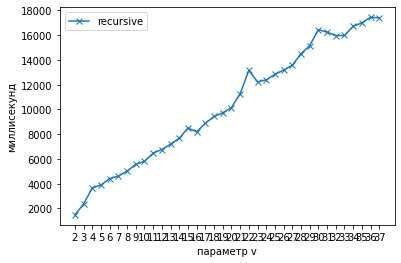
\includegraphics[width=0.6\columnwidth]{figures/vDependenceImplicitSemiLocalSARecursie.png}
    \caption{Линейная зависимость параметра рекурсивного алгоритма \emph{semi-local sa} на основе умножения липких кос }\label{fig:vParam}
\end{figure}

На рис. \ref{fig:speedWindow3} представлены результаты запусков двух версий алгоритмов для решения задачи \emph{Window-Substring}: через предподсчет кос (\emph{implicit 350}) и наивный (\emph{naive 350})\footnote{Наивный алгоритм заключается в вычислении \emph{semi-local lcs} для каждого окна $(m \times n \times w)$, где $w$ --- размер окна, $m,n$ --- размеры строк.
}.



График  показывает, что алгоритм для решения задачи \emph{Window-Substring} через предподсчет кос действительно не зависит от размера окна и быстрее наивной версии.
Несмотря на это, в силу рекурсивной структуры  алгоритма решения, он не применим к большим данным.

\begin{figure}[H]
\centering
    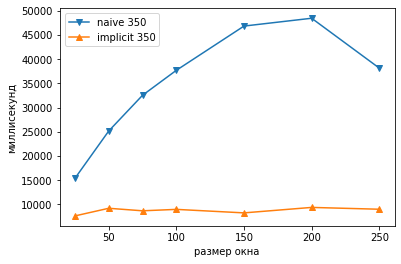
\includegraphics[width=0.6\columnwidth]{figures/windowNaiveImpl.png}
    \caption{Независимость от размера окна }\label{fig:speedWindow3}
\end{figure}

%  \linebreak[2]

Таким образом, можно сделать вывод, что  при работе с большими данными может быть эффективно применен алгоритм решения задач \emph{semi-local} через распутывание кос. 
А алгоритмы, обладающие сложной рекурсивной структурой, могут быть применены при совершении ряда оптимизаций. Например, избавления от рекурсии.

\subsection{Поиск по шаблону}
В данной секции описаны результаты запусков различных версий алгоритмов решения \emph{задачи поиска по шаблону}. Также произведен их анализ.

На рис. \ref{ssss}  представлены результаты временных замеров для  различных версий алгоритмов, решающих задачу поиска по шаблону.
В частности, алгоритм из статьи \cite{luciv2019interactive} (\emph{duplicate search}), его улучшенная версия, описанная в разделе \ref{fics} (\emph{duplicate search via semi-local}), алгоритм из \emph{библиотеки алгоритмов} (\emph{ThresholdAMatch}) и алгоритм \ref{alg:patternMathing2} с учетом замечания (см. псевдокод \ref{alg:patternMathing2}).

Рассматривались два сценария: меленький размер алфавита (большая частота повторов) и большой размер алфавита (маленькая частота повторов).
В обоих случая размер текста был фиксирован и равен \emph{10000} слов.

\begin{figure}[h]
    \centering
    \begin{subfigure}[b]{0.45\textwidth}
    \centering
    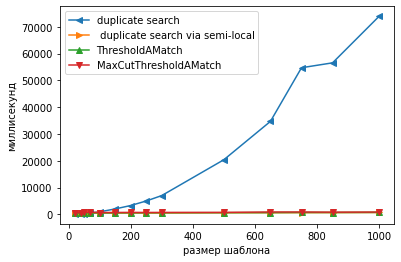
\includegraphics[width=\textwidth]{figures/smallAlphabet.png} \caption{Сценарий с малым размером\\ алфавита}
    \label{fig:subim1}
    \end{subfigure}%
    % \hfill
    \begin{subfigure}[b]{0.45\textwidth}
    \centering
    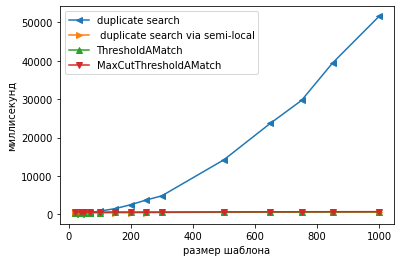
\includegraphics[width=\textwidth]{figures/largeAlphabet.png}
    \caption{Сценарий с большим размером\\ алфавита}
    \label{fig:subim2}
    \end{subfigure}
\caption{Сравнение скорости различных алгоритмов решения задачи \emph{поиска по шаблону}}\label{ssss}
\end{figure}

График, во-первых, показывает, что алгоритм решения \emph{semi-local} может быть эффективно применен к \emph{задаче поиска по образцу}, а во-вторых, что улучшенная версия алгоритма из \cite{luciv2019interactive} показывает лучшие результаты не только в теории, но и на практике.

\subsection{Поиск групп повторов}
В данной секции представлен анализ результатов запуска алгоритмов, решающих  \emph{задачу поиска групп повторов} для \emph{JavaDoc}-документа-\\ции.

Анализ производился в рамках реализованного приложения (см. главу \ref{searchPO}).
Использовались следующие фильтры: токенизация, лемматизация, удаление стоп-слов.
Повторы искались среди \emph{JavaDoc}-коммента-\\риев, относящихся к описанию методов, классов, интерфейсов.

Проекты, содержащие \emph{JavaDoc}-документацию, были выбраны на основе статей из главы \ref{duplicateReport}.

Для нахождения групп использовался алгоритм \ref{alg:groupDuplicate}.
В качестве функции $g$ были выбраны алгоритмы из \emph{библиотеки алгоритмов}, решающие задачи \emph{bounded-length Smith-Waterman} и \emph{semi-local sa}.
В качестве $s$ использовались алгоритм \ref{alg:clusterMcl} и алгоритм из \cite{tofigh2009optimum}.

Результаты представлены в таблице \ref{table}.


\begin{figure}[h]

\begin{center}
 \begin{tabular}{ | p{3cm} | p{3cm} | p{3cm} | p{3cm} | p{3cm} |} 
 \hline
 Название  проекта & Кол-во  комментариев & Кол-во  повторов & Кол-во групп & Время исполнения (сек) \\
 \hline
  slf4j & 188 & 157 & 25 & 8 \\
  \hline
  apache commons io & 1284 & 1180 & 92 & 569 \\
  \hline
  apache commons collection & 610 &495 &50 & 408 \\
  \hline
  gson & 498 & 356 & 81 & 96 \\
  \hline junit & 680 & 539 & 87 & 163 \\
  \hline mockito & 2979 & 2812 & 164 & 2012\\
  \hline guava & 4340 & 3662 & 418 & 8505 \\
  \hline
\end{tabular}
\end{center}
\caption{Результат работы приложения}\label{table}
\end{figure}
Пример группы одного из проектов представлен на рис. \ref{fig:groupViz}.

Анализ проектов с помощью приложения показал следующее.

Во-первых, построение полного графа похожести --- очень долгая операция.
Необходима предварительная фильтрация, чтобы сократить количество ребер в графе. 

Во-вторых, анализ найденных  групп показал, что они преимущественно состоят из одинаковых фрагментов (одинаковые методы, схожая функциональность) с незначительными изменениями (в графе это клики).
Сложная структура дерева (без учета клик) практически не присутствует.

В-третьих, графовые алгоритмы можно применять в задаче \emph{поиска групп повторов}.

В-четвертых, алгоритмы на основе решения задач \emph{semi-local} также могут быть успешно применены к задаче \emph{поиска групп повторов}.

В-пятых, количество повторов в \emph{JavaDoc}-документации существенно, что подтверждает результаты из статей (см. главу \ref{duplicateReport}).
